\documentclass[11pt,a4paper]{article}

\usepackage[a4paper,margin=1in]{geometry}
\usepackage{graphicx}
\usepackage{hyperref}
\usepackage{booktabs}
\usepackage{tabularx}
\usepackage{array}

\hypersetup{
    colorlinks=true,
    linkcolor=black,
    urlcolor=blue,
    citecolor=black
}

\setlength{\parskip}{4pt}
\setlength{\parindent}{0pt}
\setlength{\tabcolsep}{5pt}
\renewcommand{\arraystretch}{1.25}
\newcolumntype{Y}{>{\centering\arraybackslash}X}
\newcolumntype{M}[1]{>{\centering\arraybackslash}m{#1}}
\hyphenpenalty=7000
\exhyphenpenalty=7000
\emergencystretch=2em

\begin{document}

\begin{center}
    {\Large \textbf{EBU6304 Software Engineering Group Project}}\\[4pt]
    2025--26\\[10pt]
    {\large \textbf{Group 54}}\\[12pt]
\end{center}

\begin{tabular}{llll}
Member 1 QM no: & 231225339 & Name: & Lechen Ning \\
Member 2 QM no: & 231225557 & Name: & Lingxiang Mei \\
Member 3 QM no: & 231225672 & Name: & Siying Li \\
Member 4 QM no: & 231225270 & Name: & Zijun Song \\
Member 5 QM no: & 231225731 & Name: & Zijie Zhang \\
Member 6 QM no: & 231225649 & Name: & Zhenkun Li \\
\end{tabular}

\vspace{10pt}

\begin{center}
    {\Large \textbf{Final Short Report}}
\end{center}

\section{Design}

\subsection{Design strategy}

The project was designed as a lightweight web-based Teaching Assistant recruitment management system for BUPT International School. The main design goal was to support the complete recruitment lifecycle across three clearly separated roles: Teaching Assistant (TA), Module Organiser (MO), and Administrator (Admin). The team deliberately prioritised clarity, demonstrability, and low deployment cost over enterprise-scale complexity, because the project needed to remain understandable, testable, and easy to present within the scope of a university group assignment.

This strategy led to three main technical decisions. First, the backend was implemented using Java's built-in \texttt{HttpServer} rather than a heavyweight framework, which kept request handling explicit and easy to trace. Second, the frontend was implemented using static HTML, CSS, and JavaScript pages with a shared client utility layer, which reduced coupling and made role-based interfaces easy to organise. Third, structured project data was persisted in JSON files instead of a relational database. This reduced environment setup overhead, made stored entities transparent for inspection, and allowed user stories to be mapped directly to handlers, models, and data files.

The design also followed several practical principles. Role separation was treated as a first-class concern, because the system includes different permissions and responsibilities for applicants, instructors, and administrators. Modularity was used to keep authentication, recruitment, application, notification, upload, and administrative features maintainable. Reuse was encouraged through a shared frontend API layer and a central \texttt{DataService}. Finally, the system was designed for incremental extension, so that core workflows could be completed first and governance features could be added later without restructuring the whole codebase.

The main trade-off was between engineering transparency and industrial scalability. A Spring Boot implementation with a relational database would offer stronger production readiness, but it would also introduce configuration and deployment overhead that was unnecessary for the assessed prototype. The chosen design therefore favoured explicit control over request handling, role checks, and JSON persistence, while acknowledging that a production version would require stronger concurrency control, database transactions, and more mature security hardening.

\subsection{Architecture and component design}

The system follows a layered client-server architecture. The presentation layer contains three role-oriented portals under the \texttt{TA/}, \texttt{MO/}, and \texttt{admin/} directories. These pages rely on shared request and authentication logic in \texttt{js/api.js}, which standardises token handling, API calls, logout, notifications, and user feedback. This reduces duplication across pages and helps keep the interfaces consistent even though they serve different user groups.

\begin{figure}[!htbp]
    \centering
    \makebox[\textwidth][c]{%
        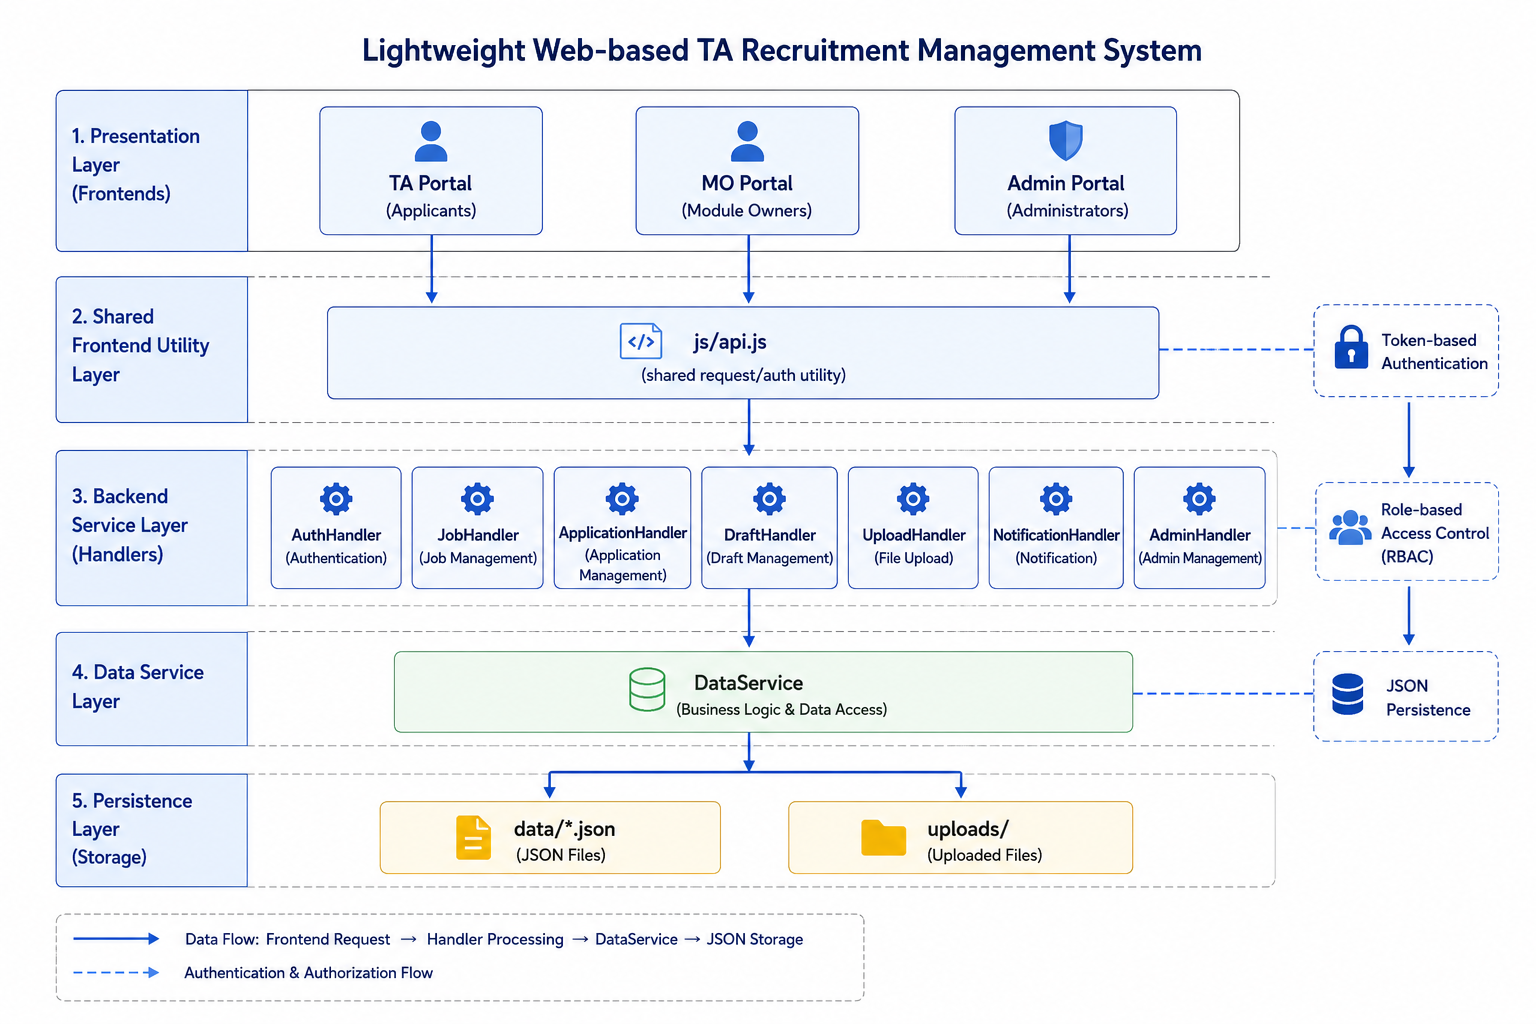
\includegraphics[width=1.08\textwidth, trim=18 18 18 18, clip]{figure/Overall system architecture diagram.png}%
    }
    \vspace{-4pt}
    \caption{Overall system architecture of the TA recruitment platform.}
\end{figure}

The business layer is composed of dedicated handler classes. \texttt{AuthHandler} manages login, registration, profile update, password change, and password reset requests. \texttt{JobHandler} supports vacancy browsing, creation, editing, and application submission. \texttt{ApplicationHandler} manages application queries, approval or rejection actions, and withdrawal. \texttt{DraftHandler} stores incomplete TA applications for later continuation. \texttt{UploadHandler} handles PDF resume upload and download. \texttt{NotificationHandler} manages user-facing notifications. \texttt{AdminHandler} groups governance functions such as user management, system statistics, workload monitoring, password reset processing, audit log review, and export tasks.

The persistence layer is centred on \texttt{DataService}. Instead of letting handlers manipulate files directly, \texttt{DataService} centralises JSON read and write operations, session lookup, draft storage, and directory initialisation. This keeps the handlers focused on request parsing and business rules while providing a single place to manage consistency of users, jobs, applications, notifications, settings, audit records, and uploaded files.

Cross-layer consistency was maintained by assigning each layer a clear responsibility. The shared \texttt{js/api.js} utility standardises token submission and API calls, handlers enforce authentication and role checks, and \texttt{DataService} centralises persistent state updates. This reduces duplicated logic and lowers the risk that different pages or handlers interpret the same workflow rule differently.

Authentication is token-based. After a successful login or registration, the server issues a session token, and the frontend stores it locally and attaches it to later requests using the \texttt{Authorization} header. On the server side, handlers resolve the token to a user identity and enforce role-based access control before executing an operation. This mechanism is relatively simple, but it is appropriate for a course project and still demonstrates explicit security logic rather than relying on hidden framework behaviour.

\subsection{Detailed design views}

At the process level, the system is organised around the TA recruitment workflow. MOs publish vacancies and configure recruitment details; TAs browse vacancies, complete applications, upload PDF resumes, save drafts, and submit final applications; the system records state changes and notifications; MOs review applicants and make decisions; and administrators supervise jobs, workload, users, audit trails, and recovery requests. This end-to-end flow shaped both page navigation and backend responsibilities.

\begin{figure}[htbp]
    \centering
    \makebox[\textwidth][c]{%
        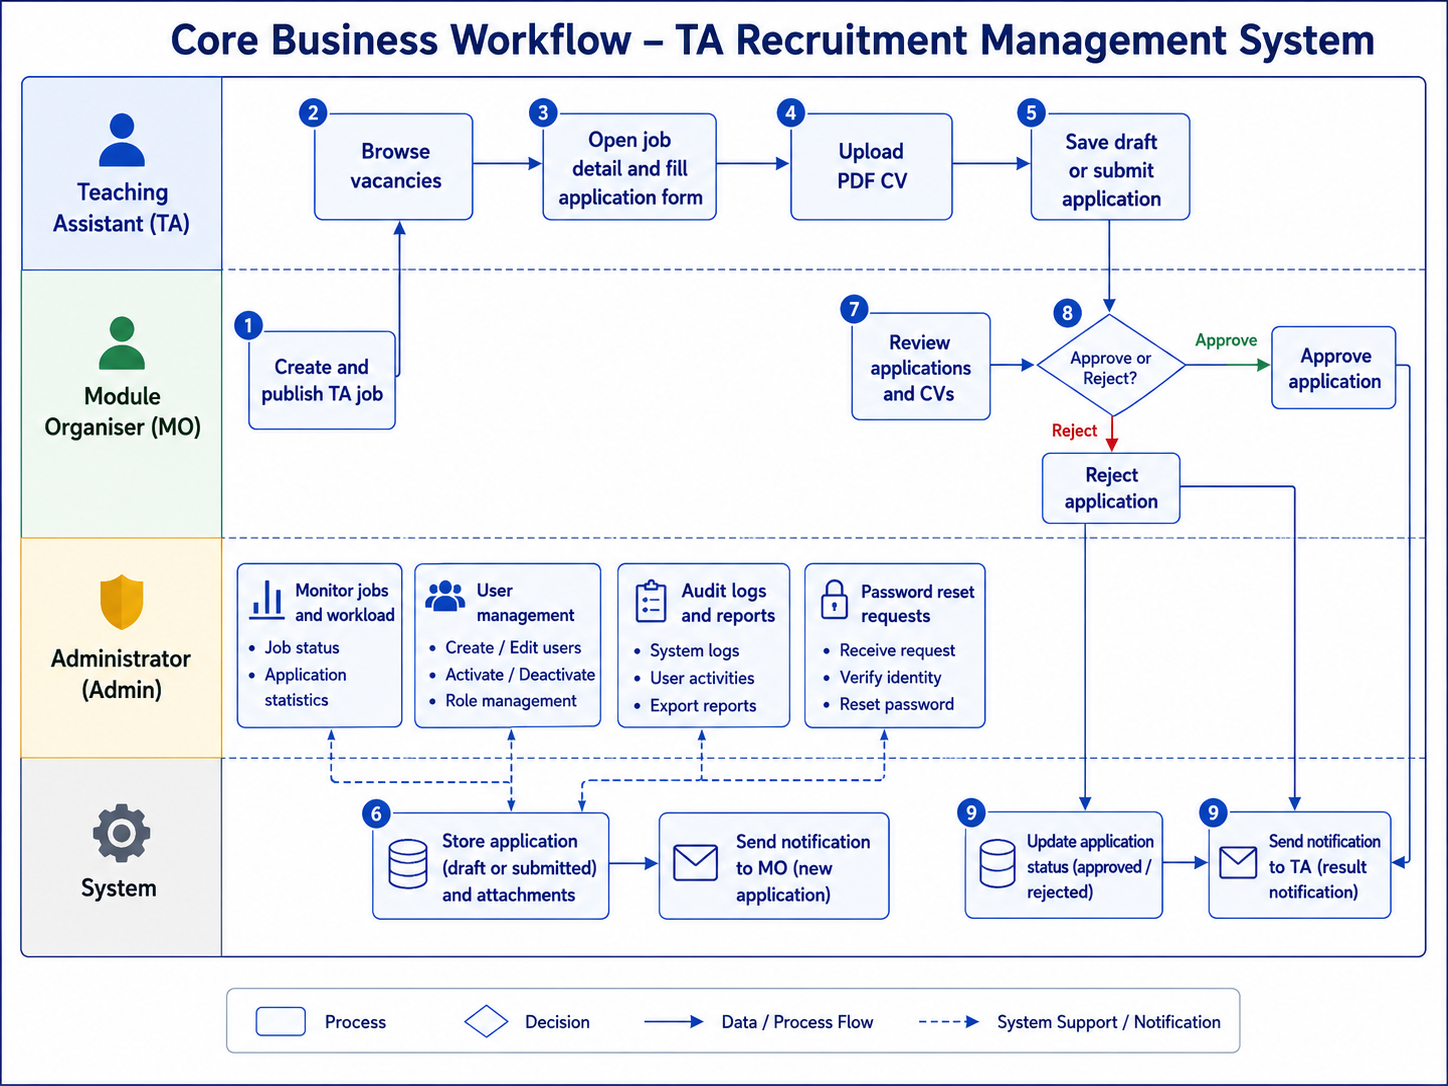
\includegraphics[width=1.14\textwidth, trim=24 22 24 22, clip]{figure/Core Business Process Diagram.png}%
    }
    \vspace{-4pt}
    \caption{Core business process across TA, MO, Admin, and system interactions.}
\end{figure}

At the data level, the core entities are \texttt{User}, \texttt{Job}, \texttt{Application}, \texttt{ApplicationDraft}, \texttt{Notification}, \texttt{AuditLog}, \texttt{PasswordResetRequest}, and \texttt{ExportTask}. These models make the stored JSON structure explicit and readable. For example, \texttt{Application} records the applicant, target job, status, priority, uploaded CV filename, timestamps, and AI-related advisory information, while \texttt{Job} stores job type, course context, quota, deadline, and workload-related scheduling details. This model set was sufficient to support the required workflow without introducing unnecessary abstraction.

\begin{figure}[htbp]
    \centering
    \makebox[\textwidth][c]{%
        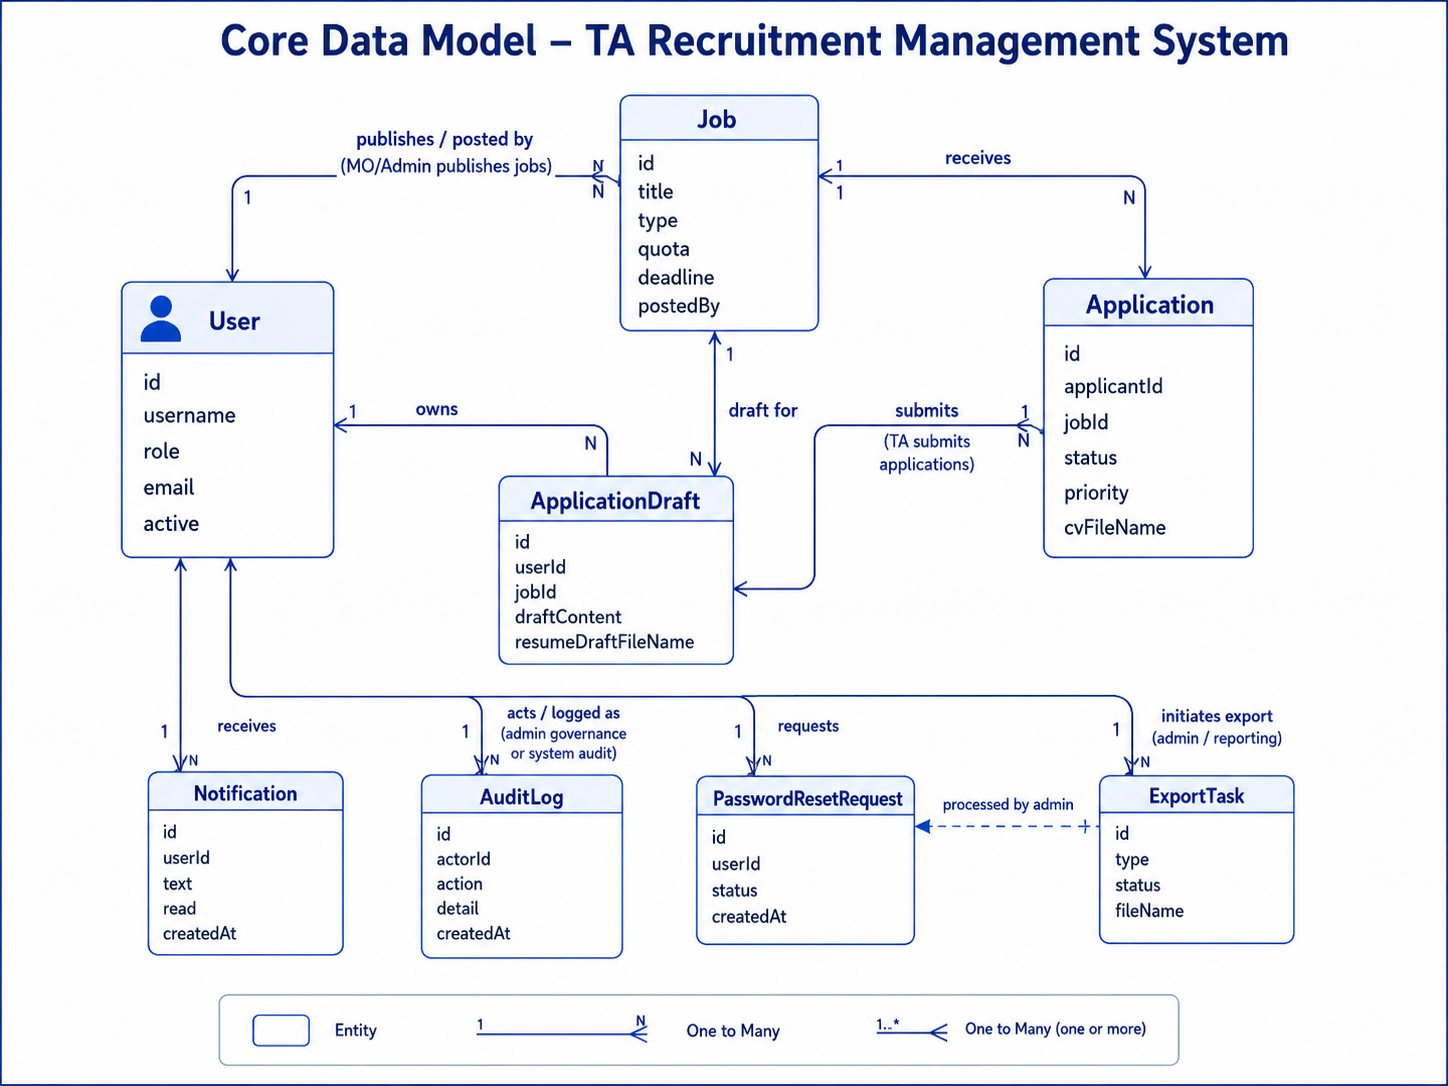
\includegraphics[width=1.10\textwidth, trim=18 4 18 14, clip]{figure/Core data model diagram.png}%
    }
    \vspace{-4pt}
    \caption{Core data model used by the recruitment system.}
\end{figure}

Several design refinements were applied during implementation. One example was the handling of TA application autofill and saved drafts. The final design scopes local draft and cached resume data to the current user rather than only to the job identifier, which prevents one TA account from loading another user's cached form data when accounts are switched in the same browser. This type of refinement reflects the general design principle used throughout the project: simple mechanisms are acceptable, but role isolation and data correctness must not be compromised.

\section{Implementation}

\subsection{Implementation strategy and project build plan}

Implementation followed an incremental strategy centred on the recruitment lifecycle. The team first built the minimum server and persistence structure, then completed the TA workflow as the main end-to-end path, then extended the system with MO-side recruitment management and Admin-side governance functions. This sequence reduced integration risk because each stage added capabilities on top of an already working core rather than opening several incomplete flows in parallel.

\begin{table}[htbp]
\centering
\small
\caption{Incremental build plan}
\begin{tabularx}{\textwidth}{M{0.10\textwidth} M{0.25\textwidth} Y}
\toprule
\textbf{Stage} & \textbf{Main focus} & \textbf{Deliverable} \\
\midrule
1 & Project skeleton & Java server startup, static file serving, authentication entry points, shared frontend API utility, and JSON persistence. \\
2 & TA workflow & Profile handling, vacancy browsing, application submission, PDF upload, draft saving, and application tracking. \\
3 & MO workflow & Job publishing and editing, applicant review, approval and rejection actions, and recruitment status management. \\
4 & Admin workflow & User management, statistics, workload monitoring, audit logs, password reset processing, and export support. \\
5 & Integration and testing & Bug fixing, usability refinement, automated tests, integration checks, and final demonstration preparation. \\
\bottomrule
\end{tabularx}
\end{table}

This plan was appropriate for a six-person team because it aligned technical delivery with functional responsibility. The TA workflow offered the shortest complete path through the system, so it served as the primary integration target. Once this path was stable, MO and Admin features could be layered onto the same models, handlers, and data service with lower coordination cost.

From a build perspective, the project remains lightweight. It uses Java 11+, a small Gson dependency, and Windows batch scripts for compilation and launch. The same Java server hosts both the APIs and the static pages, which simplifies local deployment and reduces environment mismatch between development and demonstration.

The implementation also deliberately kept the API surface aligned with the user stories. Each major workflow is represented by a small group of endpoints and a corresponding handler, which made integration easier to reason about during group development. This structure also helped later testing, because the same request boundaries used by the frontend could be exercised directly in handler-level tests.

\subsection{Version control and collaboration}

Git was used to support collaboration, traceability, and staged integration. Because the repository separates role portals, backend handlers, models, services, and tests, team members could work on different functional slices with relatively low merge conflict risk. Commits were linked to identifiable increments such as draft recovery, upload validation, statistics pages, AI matching, and password reset processing.

Version control also supported quality management. It allowed the group to compare intermediate versions, preserve stable baselines, and integrate changes gradually instead of through a single final merge. This was especially useful in a role-based system where changes to models, request handling, or permissions can affect several workflows at once.

\section{Testing}

\subsection{Testing strategy}

The testing strategy focused on correctness of business rules, access control, persistence behaviour, and side effects. Since the system is organised around HTTP handlers and shared services, the most effective test target was the handler/API level rather than isolated page widgets. This allowed the tests to exercise realistic request paths while keeping execution fast and reproducible.

Handler/API-level tests provided stronger evidence than page screenshots alone because they verified permissions, state transitions, JSON side effects, notifications, and audit records at the same boundary used by the running system. However, this does not remove the need for future browser end-to-end tests for layout, popup behaviour, and cross-browser interaction.

\begin{table}[htbp]
\centering
\footnotesize
\caption{Testing strategy matrix}
\begin{tabularx}{\textwidth}{M{0.23\textwidth} M{0.25\textwidth} Y}
\toprule
\textbf{Risk area} & \textbf{Testing technique} & \textbf{Example scenarios} \\
\midrule
Authentication and session control & Handler-level request simulation & Login, registration, token resolution, and unauthenticated access rejection. \\
Role-based access control & Role-scoped API tests & TA-only submission, MO-only job management, and Admin-only governance operations. \\
Application workflow rules & Story-based unit/API tests & Duplicate application blocking, priority limits, withdrawal, approval, and rejection transitions. \\
JSON persistence & Temporary-directory data isolation & User, job, draft, notification, and application updates written and reloaded correctly. \\
Upload handling & File upload and retrieval tests & PDF validation, stored filename reuse, and download correctness. \\
Notification and audit side effects & Response and persistence assertions & Notification creation after actions and audit log recording for sensitive operations. \\
AI Match constraints & Boundary and validation tests & Unsupported model rejection, usage-limit enforcement, and structured result generation. \\
Admin governance functions & Admin workflow tests & Password reset review, workload statistics, user management, and export-related operations. \\
\bottomrule
\end{tabularx}
\end{table}

The automated tests were written in JUnit 5. A custom \texttt{TestHttpExchange} helper simulated HTTP requests and responses, while temporary folders isolated test data from the main project files. This approach was particularly effective for validating request handling, JSON persistence, notification creation, and role-specific behaviour without relying on manual browser interaction.

\subsection{Test results}

According to the latest evidence recorded in \texttt{UNIT\_TEST\_EVIDENCE.md}, the automated suite found 70 tests and all 70 passed successfully, with 0 failures. This result indicates that the current backend and handler logic satisfies the scenarios covered by the implemented tests.

\begin{table}[htbp]
\centering
\small
\caption{Summary of latest automated test evidence}
\begin{tabularx}{0.82\textwidth}{M{0.35\textwidth} Y}
\toprule
\textbf{Item} & \textbf{Result} \\
\midrule
Test framework & JUnit 5 \\
Test style & Handler/API-level tests \\
Tests found & 70 \\
Tests successful & 70 \\
Tests failed & 0 \\
Key coverage & Authentication, jobs, applications, drafts, uploads, AI matching, and admin operations \\
\bottomrule
\end{tabularx}
\end{table}

The evidence is strong at the backend behaviour level, but it does not fully replace manual verification of browser rendering, popup preview behaviour, or live external services such as real email delivery and production AI API availability. In that sense, the testing strategy provides credible engineering evidence for functional correctness, while leaving room for future end-to-end testing.

The main residual testing risk is therefore not the absence of unit evidence, but the absence of a full browser automation layer. A production-oriented continuation would add end-to-end tests for the highest-value journeys: TA submission, MO review, Admin password reset processing, and AI Match display behaviour across browsers.

\section{The use of Generative AI (GenAI)}

\subsection{GenAI during development}

Generative AI was used as a development support tool rather than as a substitute for engineering judgement. During implementation, AI assistance was used to diagnose bugs, suggest implementation patterns, accelerate repetitive coding tasks, and propose alternatives for practical development problems. This was especially useful when the team was still learning some web-development techniques and needed quick guidance on frontend interaction, request handling, and cross-layer integration.

The main benefit of GenAI during development was iteration speed. It was effective for producing candidate code snippets, identifying likely causes of bugs, and offering refactoring suggestions. However, AI output still required careful human review because proposals were not always fully aligned with the project data model, role constraints, or persistence design.

\subsection{GenAI inside the system}

GenAI was also integrated into the system itself through the AI Match Assistant. This feature compares an applicant's profile and motivation text with the requirements of a TA vacancy. On the TA side, it presents a match score, matched skills, missing skills, recommendation text, and workload cues. On the MO side, it provides a compact summary to support applicant review.

\begin{figure}[htbp]
    \centering
    \begin{minipage}[t]{0.39\textwidth}
        \centering
        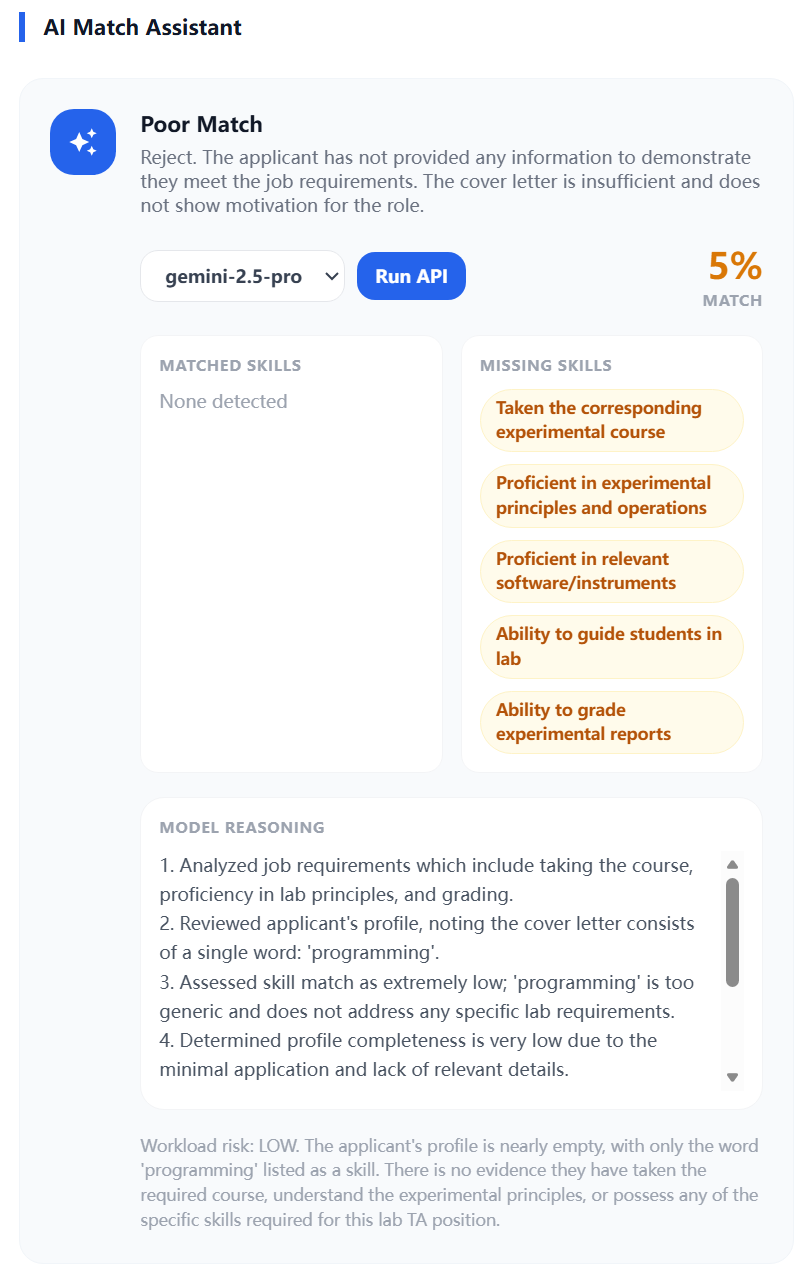
\includegraphics[width=\textwidth]{figure/Interface diagram of AI Match function_TA.png}
        \vspace{-2pt}
        \footnotesize Figure 4(a). TA-side AI Match Assistant.
    \end{minipage}
    \hfill
    \begin{minipage}[t]{0.39\textwidth}
        \centering
        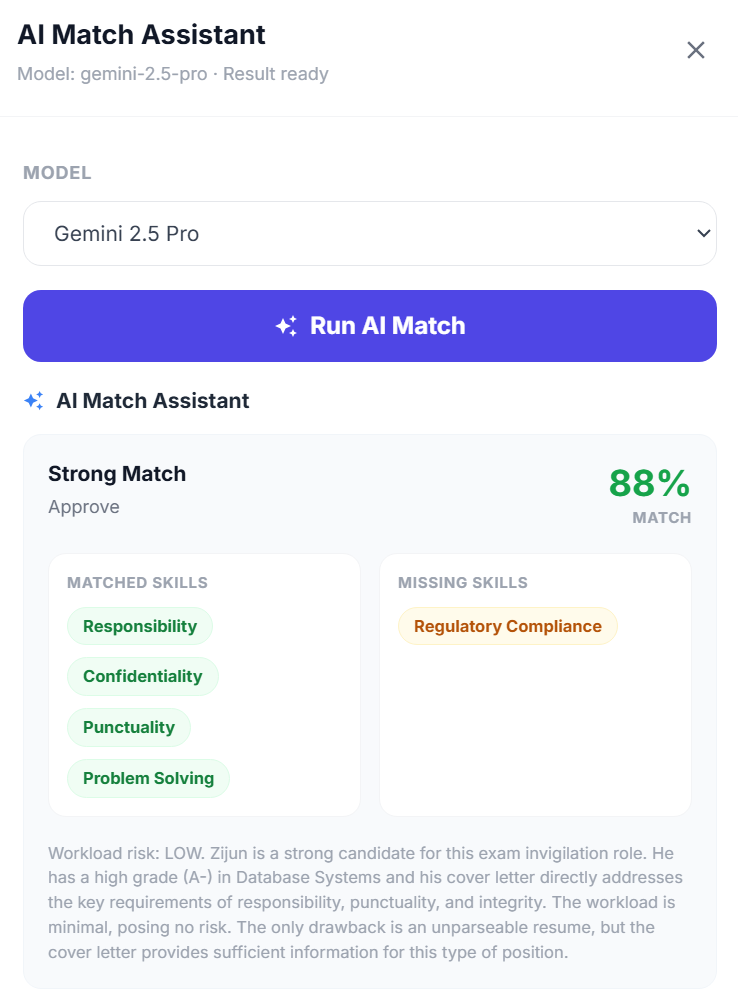
\includegraphics[width=\textwidth]{figure/Interface diagram of AI Match function_MO.png}
        \vspace{-2pt}
        \footnotesize Figure 4(b). MO-side AI match summary.
    \end{minipage}
    \vspace{-3pt}
    \caption{AI Match interfaces for the TA and MO portals.}
\end{figure}

The AI Match Assistant is designed as a decision-support feature, not an autonomous decision-maker. Final approval remains with the human MO reviewer. The system also constrains model selection and usage limits, and its recommendations are presented as explainable guidance only. This is important because AI output may be incomplete, biased, or weakened by poor applicant input even when the generated explanation appears plausible.

The human-in-the-loop design is also an ethical control. AI Match can help organise evidence, but it may hallucinate, over-emphasise weak signals, or reflect bias in incomplete applicant input. The MO reviewer therefore remains accountable for the decision, and the AI result is treated as advisory evidence rather than a ranking authority.

\subsection{Limitations and challenges}

The project also exposed broader limitations of GenAI. AI suggestions can sound confident even when based on incomplete evidence, and external AI APIs introduce operational uncertainty such as latency, rate limits, and inconsistent output quality. As a result, GenAI was valuable in this project both as a development accelerator and as a product feature, but in both roles it required explicit human oversight and clear operational boundaries.

\clearpage
\section*{Individual Statements}

The following individual statements are submitted separately from the group report body. Each statement is kept within the 300-word limit.

{\sloppy

\textbf{QM no: 231225339}\\
\textbf{Name: Lechen Ning}\\
\textbf{Main contribution:} I was mainly responsible for project planning, initial framework construction, Git-based collaboration management, and part of the Admin supervision views. My work helped establish the overall project structure, development workflow, and implementation direction before different members extended their own functional modules. I also contributed to the administrative monitoring side, where the system needed to present management information clearly for supervision and review.\\
\textbf{Reflective statement:} This project improved my understanding of how planning and architecture influence later implementation. I learned that a group project requires not only coding ability, but also early decisions about structure, responsibilities, and integration workflow. Managing the project framework and Git collaboration made me more aware of the importance of stable baselines, clear module boundaries, and incremental integration. Working on Admin supervision views also helped me understand how management users need concise, reliable, and well-organised information rather than only basic CRUD functions.

\vspace{6pt}

\textbf{QM no: 231225557}\\
\textbf{Name: Lingxiang Mei}\\
\textbf{Main contribution:} I was mainly responsible for frontend interface construction, the MO-side job management workflow, and the AI Match function. My work covered the design and implementation of user-facing pages, the workflow for Module Organisers to create, edit, view, and manage TA jobs, and the integration of AI-assisted matching as a decision-support feature. I also helped connect frontend interactions with backend logic so that job management and AI Match results could be used smoothly in the recruitment process.\\
\textbf{Reflective statement:} Through this project, I gained a stronger understanding of how frontend design, workflow logic, and backend data interaction need to work together. The MO-side job management process taught me that even a simple-looking interface requires careful handling of state, validation, permissions, and user feedback. Implementing AI Match also made me think more critically about the role of GenAI in software systems. I learned that AI should not replace human judgement, but it can provide useful support when its output is constrained, explainable, and clearly positioned as advisory.

\vspace{6pt}

\textbf{QM no: 231225672}\\
\textbf{Name: Siying Li}\\
\textbf{Main contribution:} I was mainly responsible for the TA-side application workflow, TA-facing interface support, and unit testing. My work focused on the applicant experience, including browsing recruitment information, completing application forms, interacting with application-related pages, and supporting the correctness of the workflow through tests. I also contributed to interface usability, form behaviour, validation logic, and test cases that helped verify the reliability of TA-side operations.\\
\textbf{Reflective statement:} This project gave me practical experience in turning user requirements into concrete interface behaviour and testable functions. Working on the TA-side workflow showed me that applicant-facing features must be clear, reliable, and easy to follow, because they directly affect whether users can complete the recruitment process successfully. Unit testing also changed how I think about software quality. Instead of only checking whether a page looks correct, I learned to consider edge cases, workflow assumptions, permission boundaries, and persistent data changes. This strengthened both my frontend implementation skills and my awareness of quality assurance.

\vspace{6pt}

\textbf{QM no: 231225270}\\
\textbf{Name: Zijun Song}\\
\textbf{Main contribution:} I was mainly responsible for Admin governance functions, the login interface, and password reset processing. My work focused on administrative control and system access, including user-related governance, security-related workflows, login interaction, and recovery mechanisms for password reset requests. These functions helped ensure that the system was not only usable for recruitment, but also manageable and controllable from an administrator perspective.\\
\textbf{Reflective statement:} Working on the governance and access-control side of the system helped me understand that administration features are essential for maintaining trust and reliability. Login and password reset workflows seem common, but they require careful design because they directly affect security and user access. Admin governance also made me more aware of the need for traceability, permission separation, and consistent handling of sensitive operations. This project improved my ability to think beyond visible page functions and consider how a system should be controlled, recovered, and maintained after deployment.

\vspace{6pt}

\textbf{QM no: 231225731}\\
\textbf{Name: Zijie Zhang}\\
\textbf{Main contribution:} I was mainly responsible for the MO-side interface, message sending, and notification-related functions. My work supported the Module Organiser experience by helping users interact with job-related information, communicate system updates, and receive or send recruitment-related messages. These functions contributed to the coordination between job management, application review, and user communication within the recruitment process.\\
\textbf{Reflective statement:} This project helped me understand the importance of communication features in a management system. A recruitment platform is not only about storing jobs and applications; it also needs to keep different users informed at the right time. Working on the MO interface and notification-related functions made me pay more attention to clarity, timing, and consistency of user feedback. I also learned that interface design should support the user's working context. For Module Organisers, the system needs to make job information, messages, and recruitment updates easy to access and act upon.

\vspace{6pt}

\textbf{QM no: 231225649}\\
\textbf{Name: Zhenkun Li}\\
\textbf{Main contribution:} I was mainly responsible for Admin-side data presentation. My work focused on presenting administrative information in a clear and useful way, including data views that support supervision, monitoring, and decision-making. This contribution helped the Admin role understand the system status, review relevant information, and manage the recruitment platform from a broader operational perspective.\\
\textbf{Reflective statement:} Working on Admin data presentation helped me understand that management users need information to be organised, comparable, and easy to interpret. Unlike applicant-facing pages, Admin views must support supervision and decision-making rather than only task completion. This required me to think carefully about what data should be displayed, how it should be structured, and how the interface could reduce the user's effort in understanding system status. Through this work, I improved my awareness of data-driven interface design and the relationship between backend records and management-level presentation.

}

\end{document}
